% Neural network diagram
% Made with Xematics. Positions are in px (1 px = 0.75 pt), as in the SVG export.
\documentclass[tikz, border=4pt]{standalone}
\definecolor{xm1}{HTML}{FFFFFF}
\definecolor{xm2}{HTML}{F1F2F4}
\definecolor{xm3}{HTML}{4B5563}
\definecolor{xm4}{HTML}{FBE8C4}
\definecolor{xm5}{HTML}{B97800}
\definecolor{xm6}{HTML}{B8C0CC}
\definecolor{xm7}{HTML}{D4E8F5}
\definecolor{xm8}{HTML}{0072B2}
\definecolor{xm9}{HTML}{AEB3B9}
\definecolor{xm10}{HTML}{6B7280}
\definecolor{xm11}{HTML}{1F2937}
\begin{document}
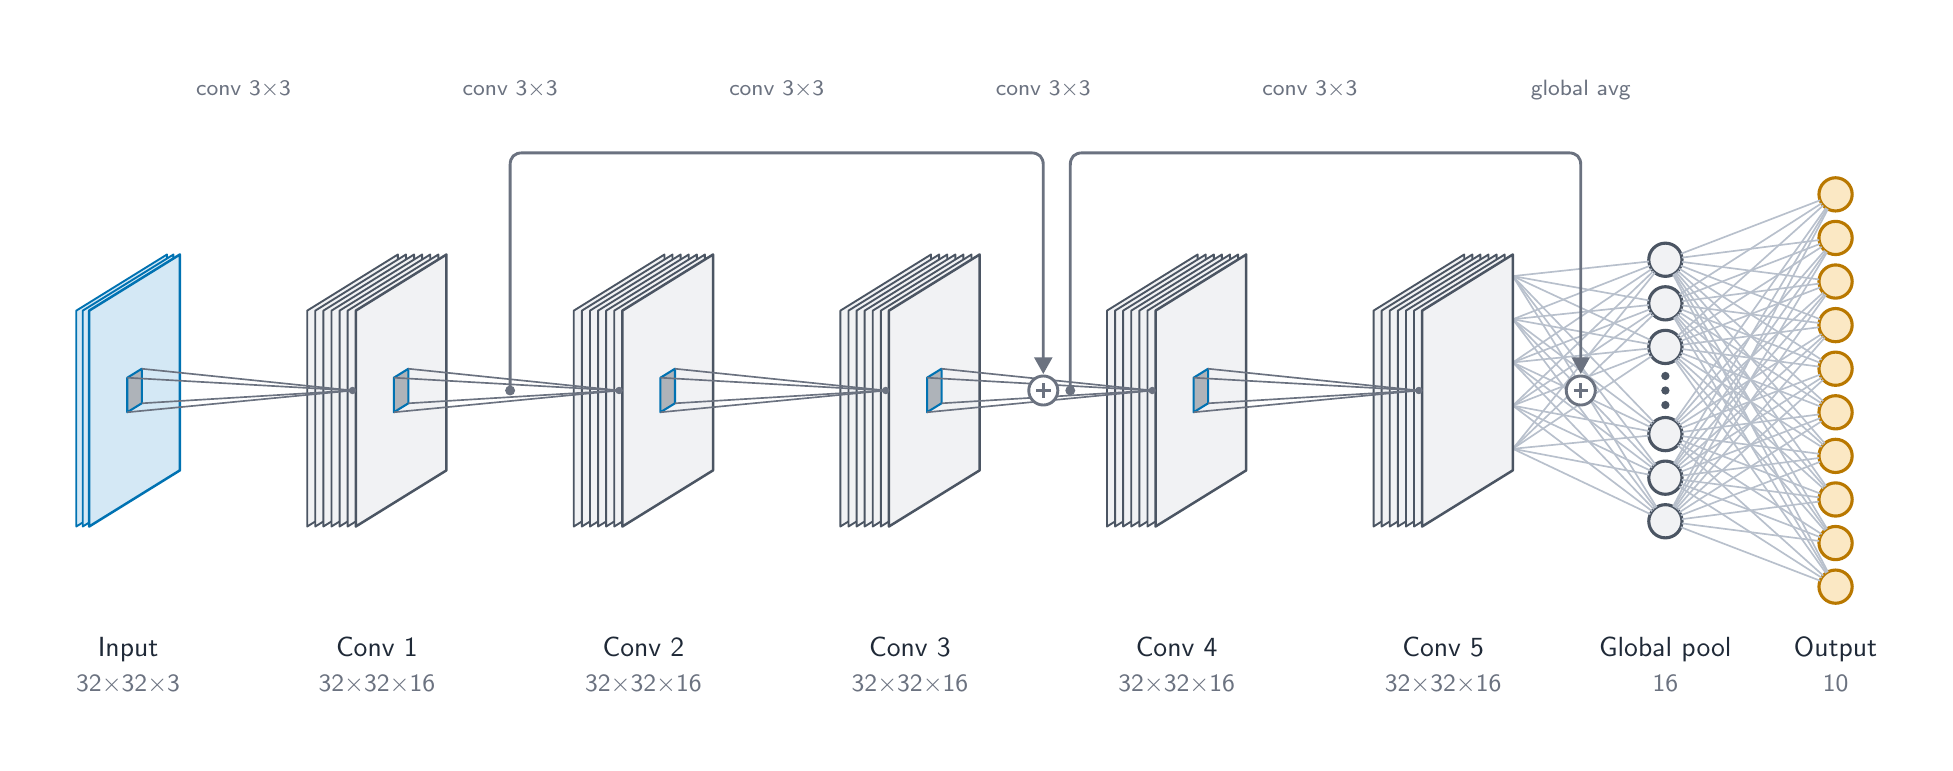
\begin{tikzpicture}[x=0.75pt, y=-0.75pt]
  \tikzset{
    xm hidden/.style={circle, minimum size=12pt, inner sep=0, outer sep=0, fill=xm2, draw=xm3, line width=1.13pt},
    xm output/.style={circle, minimum size=12pt, inner sep=0, outer sep=0, fill=xm4, draw=xm5, line width=1.13pt},
    xm edge/.style={draw=xm6, line width=0.6pt},
    xm map input back/.style={fill=xm7, draw=xm8, line width=0.68pt, line join=round},
    xm map input/.style={fill=xm7, draw=xm8, line width=0.9pt, line join=round},
    xm map hidden back/.style={fill=xm2, draw=xm3, line width=0.68pt, line join=round},
    xm map hidden/.style={fill=xm2, draw=xm3, line width=0.9pt, line join=round},
    xm dots/.style={fill=xm3},
    xm window/.style={fill=xm9, draw=xm8, line width=0.75pt, line join=round},
    xm ray/.style={draw=xm10, line width=0.6pt},
    xm ray end/.style={fill=xm10},
    xm skip start/.style={fill=xm10},
    xm skip add/.style={fill=none, draw=xm10, line width=1.05pt, line join=round},
    xm skip head/.style={fill=xm10},
    xm join/.style={fill=xm1, draw=xm10, line width=1.05pt},
    xm join sign/.style={fill=none, draw=xm10, line width=1.05pt},
    xm name xm11/.style={text=xm11, inner sep=0, font=\sffamily\fontsize{9.75}{11.7}\selectfont},
    xm size xm10/.style={text=xm10, inner sep=0, font=\sffamily\fontsize{9}{10.8}\selectfont},
    xm op xm10/.style={text=xm10, inner sep=0, font=\sffamily\fontsize{8.25}{9.9}\selectfont},
  }
  \fill[xm1] (0,0) rectangle (914.28,344.56);
  % Neurons
  \node[xm hidden] (n-6-0) at (789.04,111.81) {};
  \node[xm hidden] (n-6-1) at (789.04,132.81) {};
  \node[xm hidden] (n-6-2) at (789.04,153.81) {};
  \node[xm hidden] (n-6-13) at (789.04,195.81) {};
  \node[xm hidden] (n-6-14) at (789.04,216.81) {};
  \node[xm hidden] (n-6-15) at (789.04,237.81) {};
  \node[xm output] (n-7-0) at (871.04,80.31) {};
  \node[xm output] (n-7-1) at (871.04,101.31) {};
  \node[xm output] (n-7-2) at (871.04,122.31) {};
  \node[xm output] (n-7-3) at (871.04,143.31) {};
  \node[xm output] (n-7-4) at (871.04,164.31) {};
  \node[xm output] (n-7-5) at (871.04,185.31) {};
  \node[xm output] (n-7-6) at (871.04,206.31) {};
  \node[xm output] (n-7-7) at (871.04,227.31) {};
  \node[xm output] (n-7-8) at (871.04,248.31) {};
  \node[xm output] (n-7-9) at (871.04,269.31) {};
  % Connections 5
  \draw[xm edge] (715.52,119.69) -- (n-6-0);
  \draw[xm edge] (715.52,119.69) -- (n-6-1);
  \draw[xm edge] (715.52,119.69) -- (n-6-2);
  \draw[xm edge] (715.52,119.69) -- (n-6-13);
  \draw[xm edge] (715.52,119.69) -- (n-6-14);
  \draw[xm edge] (715.52,119.69) -- (n-6-15);
  \draw[xm edge] (715.52,140.49) -- (n-6-0);
  \draw[xm edge] (715.52,140.49) -- (n-6-1);
  \draw[xm edge] (715.52,140.49) -- (n-6-2);
  \draw[xm edge] (715.52,140.49) -- (n-6-13);
  \draw[xm edge] (715.52,140.49) -- (n-6-14);
  \draw[xm edge] (715.52,140.49) -- (n-6-15);
  \draw[xm edge] (715.52,161.29) -- (n-6-0);
  \draw[xm edge] (715.52,161.29) -- (n-6-1);
  \draw[xm edge] (715.52,161.29) -- (n-6-2);
  \draw[xm edge] (715.52,161.29) -- (n-6-13);
  \draw[xm edge] (715.52,161.29) -- (n-6-14);
  \draw[xm edge] (715.52,161.29) -- (n-6-15);
  \draw[xm edge] (715.52,182.09) -- (n-6-0);
  \draw[xm edge] (715.52,182.09) -- (n-6-1);
  \draw[xm edge] (715.52,182.09) -- (n-6-2);
  \draw[xm edge] (715.52,182.09) -- (n-6-13);
  \draw[xm edge] (715.52,182.09) -- (n-6-14);
  \draw[xm edge] (715.52,182.09) -- (n-6-15);
  \draw[xm edge] (715.52,202.89) -- (n-6-0);
  \draw[xm edge] (715.52,202.89) -- (n-6-1);
  \draw[xm edge] (715.52,202.89) -- (n-6-2);
  \draw[xm edge] (715.52,202.89) -- (n-6-13);
  \draw[xm edge] (715.52,202.89) -- (n-6-14);
  \draw[xm edge] (715.52,202.89) -- (n-6-15);
  % Connections 6
  \draw[xm edge] (n-6-0) -- (n-7-0);
  \draw[xm edge] (n-6-0) -- (n-7-1);
  \draw[xm edge] (n-6-0) -- (n-7-2);
  \draw[xm edge] (n-6-0) -- (n-7-3);
  \draw[xm edge] (n-6-0) -- (n-7-4);
  \draw[xm edge] (n-6-0) -- (n-7-5);
  \draw[xm edge] (n-6-0) -- (n-7-6);
  \draw[xm edge] (n-6-0) -- (n-7-7);
  \draw[xm edge] (n-6-0) -- (n-7-8);
  \draw[xm edge] (n-6-0) -- (n-7-9);
  \draw[xm edge] (n-6-1) -- (n-7-0);
  \draw[xm edge] (n-6-1) -- (n-7-1);
  \draw[xm edge] (n-6-1) -- (n-7-2);
  \draw[xm edge] (n-6-1) -- (n-7-3);
  \draw[xm edge] (n-6-1) -- (n-7-4);
  \draw[xm edge] (n-6-1) -- (n-7-5);
  \draw[xm edge] (n-6-1) -- (n-7-6);
  \draw[xm edge] (n-6-1) -- (n-7-7);
  \draw[xm edge] (n-6-1) -- (n-7-8);
  \draw[xm edge] (n-6-1) -- (n-7-9);
  \draw[xm edge] (n-6-2) -- (n-7-0);
  \draw[xm edge] (n-6-2) -- (n-7-1);
  \draw[xm edge] (n-6-2) -- (n-7-2);
  \draw[xm edge] (n-6-2) -- (n-7-3);
  \draw[xm edge] (n-6-2) -- (n-7-4);
  \draw[xm edge] (n-6-2) -- (n-7-5);
  \draw[xm edge] (n-6-2) -- (n-7-6);
  \draw[xm edge] (n-6-2) -- (n-7-7);
  \draw[xm edge] (n-6-2) -- (n-7-8);
  \draw[xm edge] (n-6-2) -- (n-7-9);
  \draw[xm edge] (n-6-13) -- (n-7-0);
  \draw[xm edge] (n-6-13) -- (n-7-1);
  \draw[xm edge] (n-6-13) -- (n-7-2);
  \draw[xm edge] (n-6-13) -- (n-7-3);
  \draw[xm edge] (n-6-13) -- (n-7-4);
  \draw[xm edge] (n-6-13) -- (n-7-5);
  \draw[xm edge] (n-6-13) -- (n-7-6);
  \draw[xm edge] (n-6-13) -- (n-7-7);
  \draw[xm edge] (n-6-13) -- (n-7-8);
  \draw[xm edge] (n-6-13) -- (n-7-9);
  \draw[xm edge] (n-6-14) -- (n-7-0);
  \draw[xm edge] (n-6-14) -- (n-7-1);
  \draw[xm edge] (n-6-14) -- (n-7-2);
  \draw[xm edge] (n-6-14) -- (n-7-3);
  \draw[xm edge] (n-6-14) -- (n-7-4);
  \draw[xm edge] (n-6-14) -- (n-7-5);
  \draw[xm edge] (n-6-14) -- (n-7-6);
  \draw[xm edge] (n-6-14) -- (n-7-7);
  \draw[xm edge] (n-6-14) -- (n-7-8);
  \draw[xm edge] (n-6-14) -- (n-7-9);
  \draw[xm edge] (n-6-15) -- (n-7-0);
  \draw[xm edge] (n-6-15) -- (n-7-1);
  \draw[xm edge] (n-6-15) -- (n-7-2);
  \draw[xm edge] (n-6-15) -- (n-7-3);
  \draw[xm edge] (n-6-15) -- (n-7-4);
  \draw[xm edge] (n-6-15) -- (n-7-5);
  \draw[xm edge] (n-6-15) -- (n-7-6);
  \draw[xm edge] (n-6-15) -- (n-7-7);
  \draw[xm edge] (n-6-15) -- (n-7-8);
  \draw[xm edge] (n-6-15) -- (n-7-9);
  % Layers
  \draw[xm map input back] (23.43,136.33) -- (67.11,109.29) -- (67.11,213.29) -- (23.43,240.33) -- cycle;
  \draw[xm map input back] (26.54,136.33) -- (70.22,109.29) -- (70.22,213.29) -- (26.54,240.33) -- cycle;
  \draw[xm map input] (29.64,136.33) -- (73.32,109.29) -- (73.32,213.29) -- (29.64,240.33) -- cycle;
  \draw[xm map hidden back] (134.68,136.33) -- (178.36,109.29) -- (178.36,213.29) -- (134.68,240.33) -- cycle;
  \draw[xm map hidden back] (138.58,136.33) -- (182.26,109.29) -- (182.26,213.29) -- (138.58,240.33) -- cycle;
  \draw[xm map hidden back] (142.48,136.33) -- (186.16,109.29) -- (186.16,213.29) -- (142.48,240.33) -- cycle;
  \draw[xm map hidden back] (146.38,136.33) -- (190.06,109.29) -- (190.06,213.29) -- (146.38,240.33) -- cycle;
  \draw[xm map hidden back] (150.28,136.33) -- (193.96,109.29) -- (193.96,213.29) -- (150.28,240.33) -- cycle;
  \draw[xm map hidden back] (154.18,136.33) -- (197.86,109.29) -- (197.86,213.29) -- (154.18,240.33) -- cycle;
  \draw[xm map hidden] (158.08,136.33) -- (201.76,109.29) -- (201.76,213.29) -- (158.08,240.33) -- cycle;
  \draw[xm map hidden back] (263.12,136.33) -- (306.8,109.29) -- (306.8,213.29) -- (263.12,240.33) -- cycle;
  \draw[xm map hidden back] (267.02,136.33) -- (310.7,109.29) -- (310.7,213.29) -- (267.02,240.33) -- cycle;
  \draw[xm map hidden back] (270.92,136.33) -- (314.6,109.29) -- (314.6,213.29) -- (270.92,240.33) -- cycle;
  \draw[xm map hidden back] (274.82,136.33) -- (318.5,109.29) -- (318.5,213.29) -- (274.82,240.33) -- cycle;
  \draw[xm map hidden back] (278.72,136.33) -- (322.4,109.29) -- (322.4,213.29) -- (278.72,240.33) -- cycle;
  \draw[xm map hidden back] (282.62,136.33) -- (326.3,109.29) -- (326.3,213.29) -- (282.62,240.33) -- cycle;
  \draw[xm map hidden] (286.52,136.33) -- (330.2,109.29) -- (330.2,213.29) -- (286.52,240.33) -- cycle;
  \draw[xm map hidden back] (391.56,136.33) -- (435.24,109.29) -- (435.24,213.29) -- (391.56,240.33) -- cycle;
  \draw[xm map hidden back] (395.46,136.33) -- (439.14,109.29) -- (439.14,213.29) -- (395.46,240.33) -- cycle;
  \draw[xm map hidden back] (399.36,136.33) -- (443.04,109.29) -- (443.04,213.29) -- (399.36,240.33) -- cycle;
  \draw[xm map hidden back] (403.26,136.33) -- (446.94,109.29) -- (446.94,213.29) -- (403.26,240.33) -- cycle;
  \draw[xm map hidden back] (407.16,136.33) -- (450.84,109.29) -- (450.84,213.29) -- (407.16,240.33) -- cycle;
  \draw[xm map hidden back] (411.06,136.33) -- (454.74,109.29) -- (454.74,213.29) -- (411.06,240.33) -- cycle;
  \draw[xm map hidden] (414.96,136.33) -- (458.64,109.29) -- (458.64,213.29) -- (414.96,240.33) -- cycle;
  \draw[xm map hidden back] (520,136.33) -- (563.68,109.29) -- (563.68,213.29) -- (520,240.33) -- cycle;
  \draw[xm map hidden back] (523.9,136.33) -- (567.58,109.29) -- (567.58,213.29) -- (523.9,240.33) -- cycle;
  \draw[xm map hidden back] (527.8,136.33) -- (571.48,109.29) -- (571.48,213.29) -- (527.8,240.33) -- cycle;
  \draw[xm map hidden back] (531.7,136.33) -- (575.38,109.29) -- (575.38,213.29) -- (531.7,240.33) -- cycle;
  \draw[xm map hidden back] (535.6,136.33) -- (579.28,109.29) -- (579.28,213.29) -- (535.6,240.33) -- cycle;
  \draw[xm map hidden back] (539.5,136.33) -- (583.18,109.29) -- (583.18,213.29) -- (539.5,240.33) -- cycle;
  \draw[xm map hidden] (543.4,136.33) -- (587.08,109.29) -- (587.08,213.29) -- (543.4,240.33) -- cycle;
  \draw[xm map hidden back] (648.44,136.33) -- (692.12,109.29) -- (692.12,213.29) -- (648.44,240.33) -- cycle;
  \draw[xm map hidden back] (652.34,136.33) -- (696.02,109.29) -- (696.02,213.29) -- (652.34,240.33) -- cycle;
  \draw[xm map hidden back] (656.24,136.33) -- (699.92,109.29) -- (699.92,213.29) -- (656.24,240.33) -- cycle;
  \draw[xm map hidden back] (660.14,136.33) -- (703.82,109.29) -- (703.82,213.29) -- (660.14,240.33) -- cycle;
  \draw[xm map hidden back] (664.04,136.33) -- (707.72,109.29) -- (707.72,213.29) -- (664.04,240.33) -- cycle;
  \draw[xm map hidden back] (667.94,136.33) -- (711.62,109.29) -- (711.62,213.29) -- (667.94,240.33) -- cycle;
  \draw[xm map hidden] (671.84,136.33) -- (715.52,109.29) -- (715.52,213.29) -- (671.84,240.33) -- cycle;
  \fill[xm dots] (789.04,167.81) circle[radius=2];
  \fill[xm dots] (789.04,174.81) circle[radius=2];
  \fill[xm dots] (789.04,181.81) circle[radius=2];
  \draw[xm window] (47.99,168.65) -- (54.98,164.33) -- (54.98,180.97) -- (47.99,185.29) -- cycle;
  \draw[xm ray] (47.99,168.65) -- (156.52,174.81);
  \draw[xm ray] (54.98,164.33) -- (156.52,174.81);
  \draw[xm ray] (54.98,180.97) -- (156.52,174.81);
  \draw[xm ray] (47.99,185.29) -- (156.52,174.81);
  \fill[xm ray end] (156.52,174.81) circle[radius=1.8];
  \draw[xm window] (176.43,168.65) -- (183.42,164.33) -- (183.42,180.97) -- (176.43,185.29) -- cycle;
  \draw[xm ray] (176.43,168.65) -- (284.96,174.81);
  \draw[xm ray] (183.42,164.33) -- (284.96,174.81);
  \draw[xm ray] (183.42,180.97) -- (284.96,174.81);
  \draw[xm ray] (176.43,185.29) -- (284.96,174.81);
  \fill[xm ray end] (284.96,174.81) circle[radius=1.8];
  \draw[xm window] (304.87,168.65) -- (311.86,164.33) -- (311.86,180.97) -- (304.87,185.29) -- cycle;
  \draw[xm ray] (304.87,168.65) -- (413.4,174.81);
  \draw[xm ray] (311.86,164.33) -- (413.4,174.81);
  \draw[xm ray] (311.86,180.97) -- (413.4,174.81);
  \draw[xm ray] (304.87,185.29) -- (413.4,174.81);
  \fill[xm ray end] (413.4,174.81) circle[radius=1.8];
  \draw[xm window] (433.31,168.65) -- (440.3,164.33) -- (440.3,180.97) -- (433.31,185.29) -- cycle;
  \draw[xm ray] (433.31,168.65) -- (541.84,174.81);
  \draw[xm ray] (440.3,164.33) -- (541.84,174.81);
  \draw[xm ray] (440.3,180.97) -- (541.84,174.81);
  \draw[xm ray] (433.31,185.29) -- (541.84,174.81);
  \fill[xm ray end] (541.84,174.81) circle[radius=1.8];
  \draw[xm window] (561.75,168.65) -- (568.74,164.33) -- (568.74,180.97) -- (561.75,185.29) -- cycle;
  \draw[xm ray] (561.75,168.65) -- (670.28,174.81);
  \draw[xm ray] (568.74,164.33) -- (670.28,174.81);
  \draw[xm ray] (568.74,180.97) -- (670.28,174.81);
  \draw[xm ray] (561.75,185.29) -- (670.28,174.81);
  \fill[xm ray end] (670.28,174.81) circle[radius=1.8];
  % Skip connections
  \path[xm skip start] (232.44,174.81) circle[radius=2.4];
  \draw[xm skip add] (232.44,174.81) -- (232.44,66.31) .. controls (232.44,62.31) and (234.44,60.31) .. (238.44,60.31) -- (483.32,60.31) .. controls (487.32,60.31) and (489.32,62.31) .. (489.32,66.31) -- (489.32,160.81);
  \fill[xm skip head] (489.32,166.81) -- (484.82,158.81) -- (493.82,158.81) -- cycle;
  \path[xm join] (489.32,174.81) circle[radius=7];
  \draw[xm join sign] (485.82,174.81) -- (492.82,174.81) (489.32,171.31) -- (489.32,178.31);
  \path[xm skip start] (502.32,174.81) circle[radius=2.4];
  \draw[xm skip add] (502.32,174.81) -- (502.32,66.31) .. controls (502.32,62.31) and (504.32,60.31) .. (508.32,60.31) -- (742.28,60.31) .. controls (746.28,60.31) and (748.28,62.31) .. (748.28,66.31) -- (748.28,160.81);
  \fill[xm skip head] (748.28,166.81) -- (743.78,158.81) -- (752.78,158.81) -- cycle;
  \path[xm join] (748.28,174.81) circle[radius=7];
  \draw[xm join sign] (744.78,174.81) -- (751.78,174.81) (748.28,171.31) -- (748.28,178.31);
  % Labels
  \node[xm name xm11, anchor=base] at (48.38,302.9) {Input};
  \node[xm size xm10, anchor=base] at (48.38,319.66) {32\ensuremath{\times}32\ensuremath{\times}3};
  \node[xm op xm10, anchor=base] at (104,32.66) {conv 3\ensuremath{\times}3};
  \node[xm name xm11, anchor=base] at (168.22,302.9) {Conv 1};
  \node[xm size xm10, anchor=base] at (168.22,319.66) {32\ensuremath{\times}32\ensuremath{\times}16};
  \node[xm op xm10, anchor=base] at (232.44,32.66) {conv 3\ensuremath{\times}3};
  \node[xm name xm11, anchor=base] at (296.66,302.9) {Conv 2};
  \node[xm size xm10, anchor=base] at (296.66,319.66) {32\ensuremath{\times}32\ensuremath{\times}16};
  \node[xm op xm10, anchor=base] at (360.88,32.66) {conv 3\ensuremath{\times}3};
  \node[xm name xm11, anchor=base] at (425.1,302.9) {Conv 3};
  \node[xm size xm10, anchor=base] at (425.1,319.66) {32\ensuremath{\times}32\ensuremath{\times}16};
  \node[xm op xm10, anchor=base] at (489.32,32.66) {conv 3\ensuremath{\times}3};
  \node[xm name xm11, anchor=base] at (553.54,302.9) {Conv 4};
  \node[xm size xm10, anchor=base] at (553.54,319.66) {32\ensuremath{\times}32\ensuremath{\times}16};
  \node[xm op xm10, anchor=base] at (617.76,32.66) {conv 3\ensuremath{\times}3};
  \node[xm name xm11, anchor=base] at (681.98,302.9) {Conv 5};
  \node[xm size xm10, anchor=base] at (681.98,319.66) {32\ensuremath{\times}32\ensuremath{\times}16};
  \node[xm op xm10, anchor=base] at (748.28,32.66) {global avg};
  \node[xm name xm11, anchor=base] at (789.04,302.9) {Global pool};
  \node[xm size xm10, anchor=base] at (789.04,319.66) {16};
  \node[xm name xm11, anchor=base] at (871.04,302.9) {Output};
  \node[xm size xm10, anchor=base] at (871.04,319.66) {10};
\end{tikzpicture}
\end{document}
